\documentclass{scrartcl}
\usepackage[a4paper,left=1in,right=1in,top=1.2in,bottom=1in]{geometry}
\usepackage{siunitx}
\usepackage{graphicx}
\usepackage{mathtools}
\setkomafont{disposition}{\normalfont\bfseries}
\newcommand*\diff{\mathop{}\!\mathrm{d}}
\newcommand*\Diff[1]{\mathop{}\!\mathrm{d^#1}}
\newcommand*\colvec[3][]{
    \begin{pmatrix}\ifx\relax#1\relax\else#1\\\fi#2\\#3\end{pmatrix}
}

%title
\title{Exercise 04:\\Supervised Learning}
\subtitle{Theoretical Neuroscience II}
\author{Johannes G\"atjen \and Lorena Morton}

%use these for structure/overview
\newcommand\Question{%
  \textbf{Question:}%
}
\newcommand\Answer{%
  \textbf{Answer:}%
}

\begin{document}
\maketitle

\section{Training of feed-forward connections}
\begin{figure}[h]
\centering
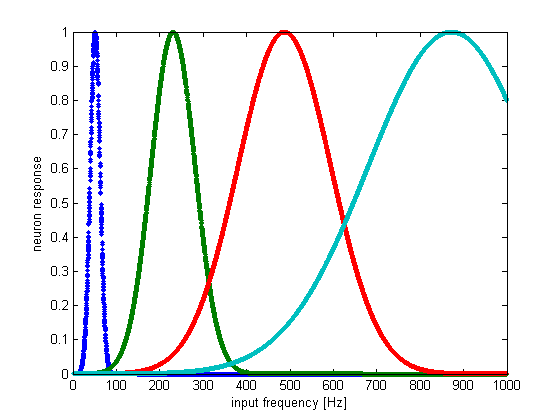
\includegraphics[trim = {0.8cm 0 0.5cm 0.2cm}, width=0.48\textwidth, clip]{../pics/lin_mean}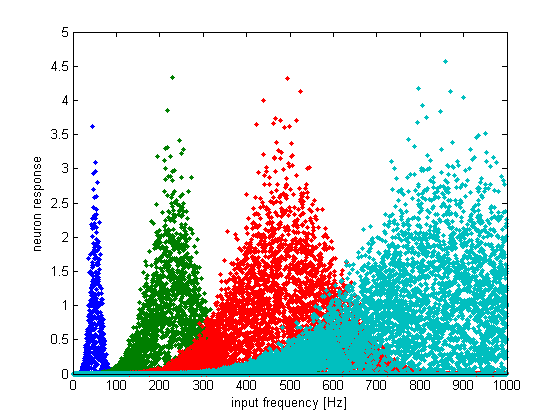
\includegraphics[trim = {0.8cm 0 0.5cm 0.2cm}, width=0.48\textwidth, clip]{../pics/lin_noise}\\
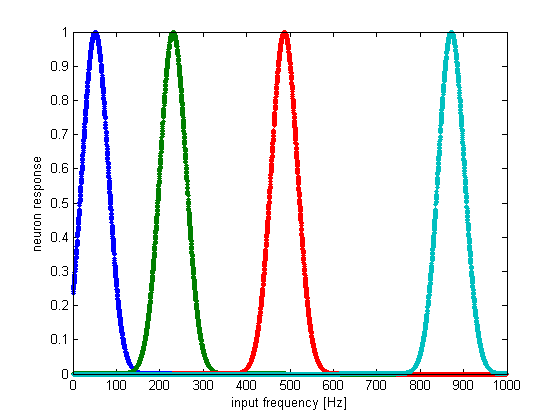
\includegraphics[trim = {0.8cm 0 0.5cm 0.2cm}, width=0.48\textwidth, clip]{../pics/cons_mean}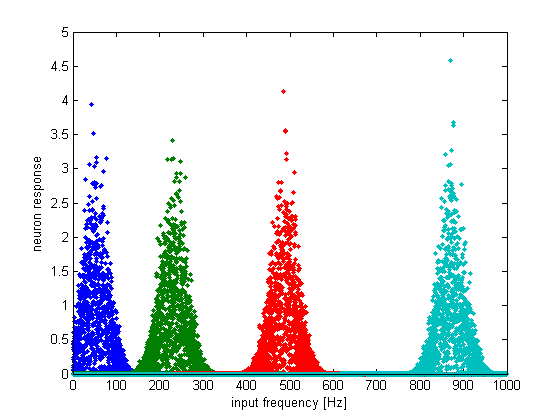
\includegraphics[trim = {0.8cm 0 0.5cm 0.2cm}, width=0.48\textwidth, clip]{../pics/cons_noise}
\caption{Left: Mean response of selected neurons to different frequencies (tuning curve). Right:~Ensemble of actual noisy responses of the same neurons. Note the larger scale on the y axis. Top: Standard deviation for tuning curve increases linearly with frequency ($\kappa = 0.22$). Bottom: Constant standard deviation ($\sigma = 30\si{Hz}$).}
\end{figure}


\begin{figure}
\centering
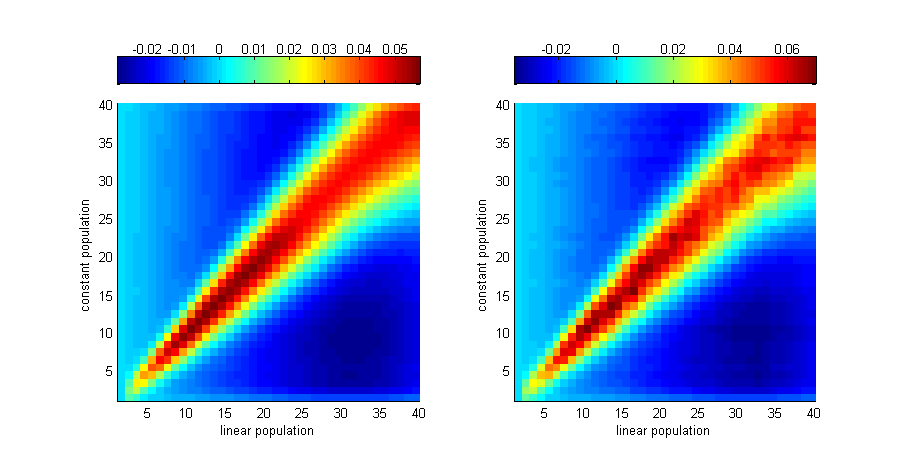
\includegraphics[trim = {1cm 0 1cm 0.3cm}, width = 0.9\textwidth, clip]{../pics/cov}
\caption{Covariance matrices for the activity of the linear and constant standard deviation populations. Left: Calculated from mean activity. Right: Calculated from noisy activity. It can be seen, that neurons close to each other are positively correlated and neurons further apart are anti-correlated.}
\end{figure}
\clearpage

\section{Decoding the downstream activity}

\begin{figure}[h]
\centering
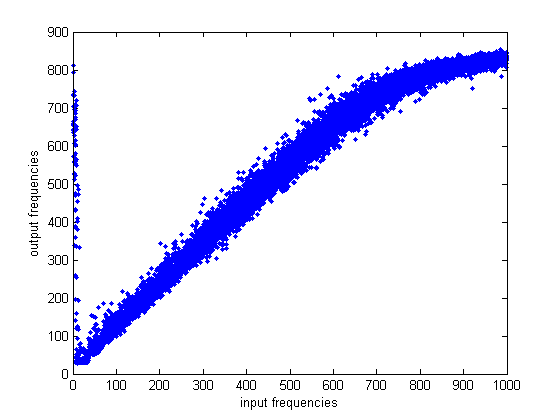
\includegraphics[trim = {0.7cm 0 0.5cm 0.2cm}, width = 0.7\textwidth, clip]{../pics/tuning}
\caption{The decoded downstream activity plotted against the input ($\sigma=30\si{Hz}$, $\kappa=0.22$, $N=M=40$). In a perfectly tuned network the points would form a straight line on the diagonal ($x=y$). Here aside from some noise, the tuning fits well for low to medium high frequency ranges. For very low inputs the decoded frequency is very inaccurate, ranging up to over 800 \si{Hz}. For inputs larger than ca.\ 750\si{Hz} the decoded frequencies are too low, due to the inaccurate input coming from the upstream population.}
\end{figure}

\begin{figure}
\centering
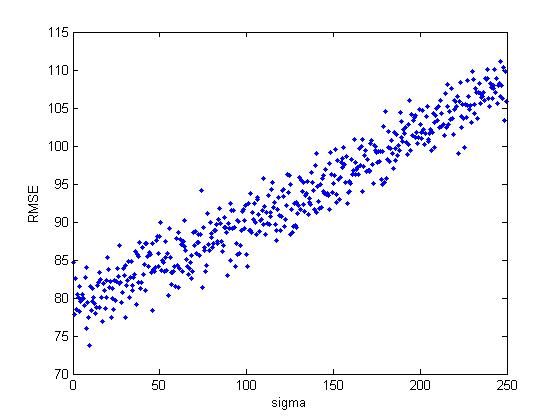
\includegraphics[trim = {0.7cm 0 0.5cm 0.2cm}, width = 0.7\textwidth, clip]{../pics/sigma}
\caption{The tuning (in)accuracy measured by the root mean square error (where error is taken as difference between input and decoded frequency) for $10000$ random inputs as a function of the $\sigma$ parameter ($\kappa=0.22$, $N=M=40$). The error grows linearly with $\sigma$.}
\end{figure}

\begin{figure}
\centering
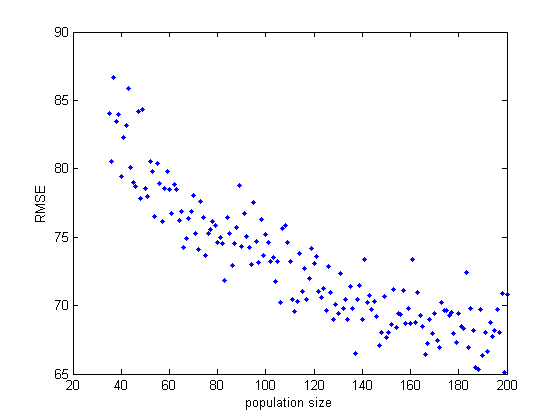
\includegraphics[trim = {0.7cm 0 0.5cm 0.2cm}, width = 0.7\textwidth, clip]{../pics/numN}
\caption{Tuning error as a function of the number of neurons in both the upstream and downstream populations ($\sigma=30\si{Hz}$, $\kappa=0.22$, $N=M$). A higher number of neurons allows slightly more accurate decoding.}
\end{figure}

\begin{figure}
\centering
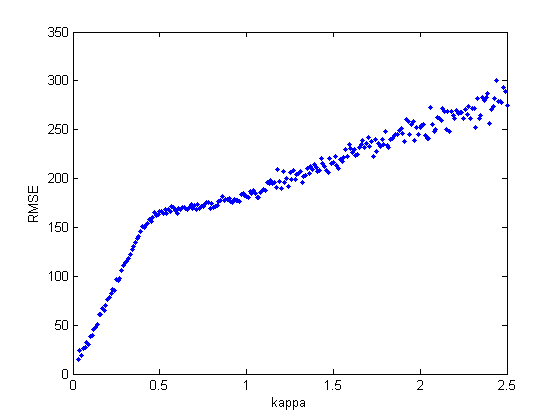
\includegraphics[trim = {0.7cm 0 0.5cm 0.2cm}, width = 0.7\textwidth, clip]{../pics/kappa}
\caption{Tuning error as a function of $\kappa$ ($\sigma=30\si{Hz}$, $N=M=40$). For $\kappa < 0.5$ the error grows quickly with increasing $\kappa$, for larger values the growth in error is less pronounced.}
\end{figure}

\end{document}